\chapter{Simplification des fonctions logiques : K-Maps}
\section{Méthodes de simplification}
Il existe différentes méthodes de simplification dont:
\begin{itemize}
	\item Via les axiomes et théorèmes déjà démontrées
	\begin{itemize}
		\item La «qualité» de l'expression obtenue dépend fortement de la capacité de manipulation des axiomes et théorèmes.
	\end{itemize}
	\item Tables de Karnaugh
	\begin{itemize}
		\item Méthode graphique rendant la simplification plus aisée. Utilisée pour des problèmes à peu de variables (max. 5).
	\end{itemize}
	\item Méthode de Quine-McCluskey
	\begin{itemize}
		\item Méthode systématique permettant de trouver l'expression la plus simple. Facile à automatiser et peut résoudre des problèmes à beaucoup de variables
	\end{itemize}
\end{itemize}
\section{Tables de Karnaugh}
La K-Map est une représentation graphique en 2D des $n$-cubes.
\begin{figure}[H]
	\begin{minipage}{0.5\textwidth}
		\centering
		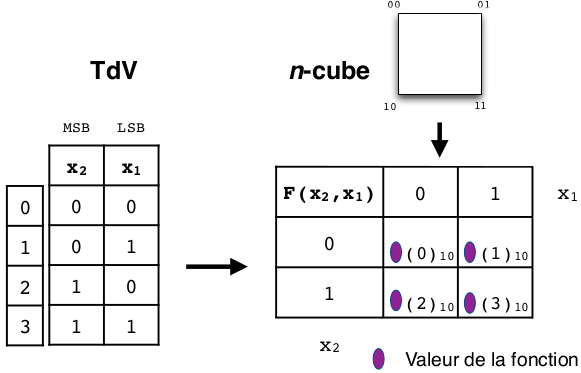
\includegraphics[width=\textwidth]{ch4/image1}
	\end{minipage}
	\begin{minipage}{0.5\textwidth}
		\centering
		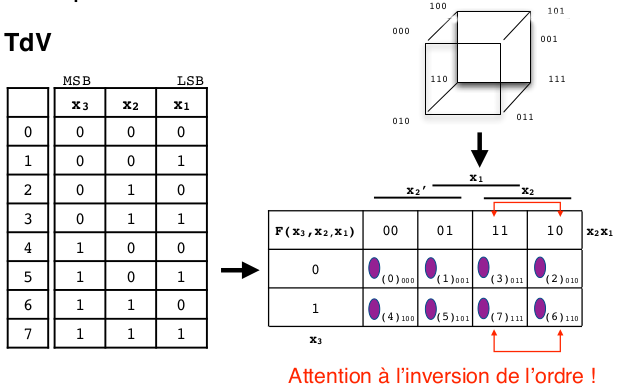
\includegraphics[width=\textwidth]{ch4/image2}
	\end{minipage}\vspace{1cm}
	\begin{minipage}{0.5\textwidth}
		\centering
		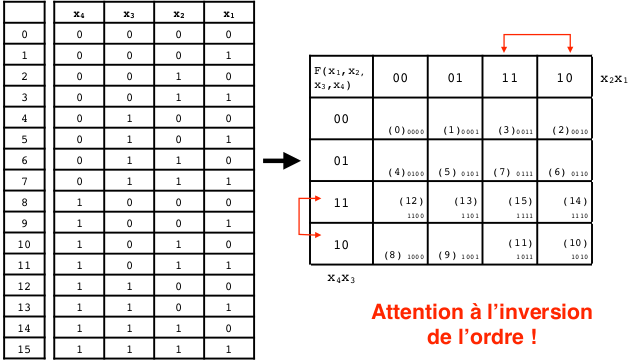
\includegraphics[width=\textwidth]{ch4/image3}
	\end{minipage}
	\begin{minipage}{0.5\textwidth}
		\centering
		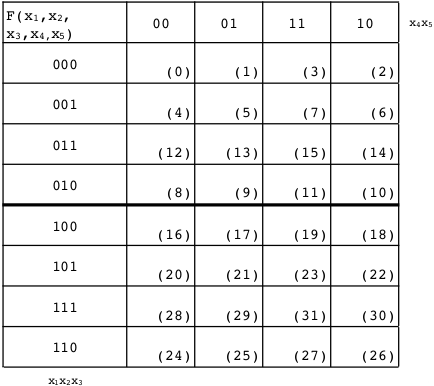
\includegraphics[width=\textwidth]{ch4/image4}
	\end{minipage}
\end{figure}
La barre en gras pour 5 variables sert à représenter la profondeur. Il faut voir la partie du haut et la partie du bas comme superposée.\\
\danger\ Ne pas oublier d'inverser $10$ et $11$ car sinon, on perd la notion de sommets adjacents (distances de Hamming seront $>1$)
\subsection{Notion de sous-cube dans un n-cube}
Une sous-cube dans un $n$-cube est un ensemble de $2^m$ sommets ($\in$ une arrête, face,\dots) pour lesquels $n-m$ variables restantes ont la même valeur.
\begin{figure}[H]
	\centering
	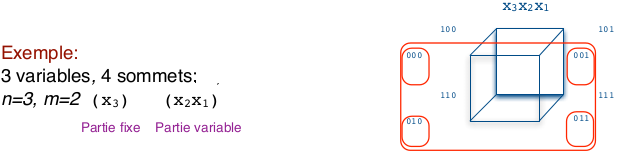
\includegraphics[width=\textwidth]{ch4/image5}
\end{figure}
Utilité ?\\
Prenons un sous-cube comprenant les sommets $000$ et $100$ correspondant à $x_1'x_2'x_3'$ et $x_1x_2'x_3'$. Si la foction logique vaut 1 à ces sommets alors:
\begin{equation}
	F=x_1'x_2'x_3'+x_1x_2'x_3' = (x_1'+x_1)x_2'x_3'=x_2'x_3'
\end{equation}
Comme définit plus haut, un sous-cube ne peut être que de taille $2^m$.
\subsubsection{Sous-cube de taille 2}
	\begin{figure}[H]
		\begin{minipage}{.5\textwidth}
			\centering
			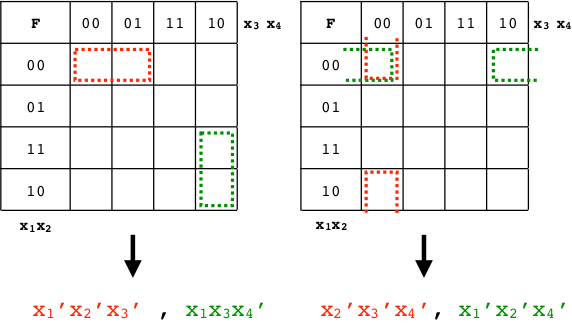
\includegraphics[width=\textwidth]{ch4/image6}
		\end{minipage}
		\begin{minipage}{.5\textwidth}
			\centering
			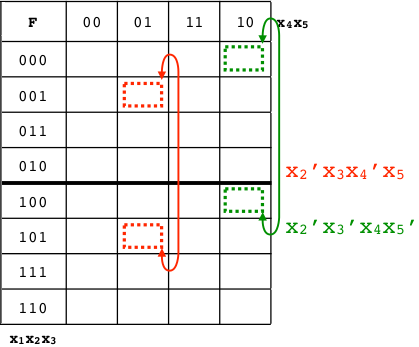
\includegraphics[width=.8\textwidth]{ch4/image7}
		\end{minipage}
	\end{figure}
\subsubsection{Sous-cube de taille 4}
	\begin{figure}[H]
		\begin{minipage}{.5\textwidth}
			\centering
			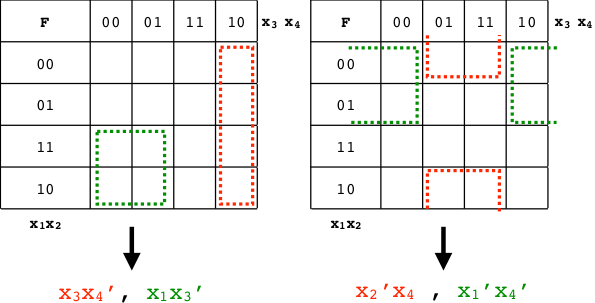
\includegraphics[width=\textwidth]{ch4/image8}
		\end{minipage}
		\begin{minipage}{.5\textwidth}
			\centering
			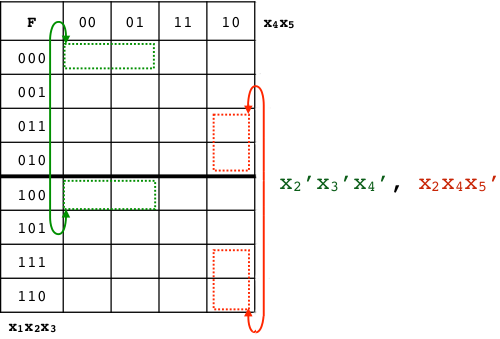
\includegraphics[width=\textwidth]{ch4/image9}
		\end{minipage}
	\end{figure}
\subsubsection{Sous-cube de taille 8}
	\begin{figure}[H]
		\begin{minipage}{.5\textwidth}
			\centering
			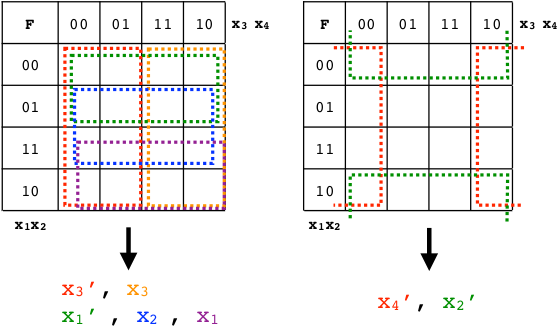
\includegraphics[width=\textwidth]{ch4/image10}
		\end{minipage}
		\begin{minipage}{.5\textwidth}
			\centering
			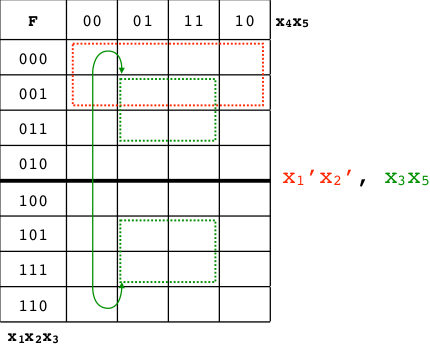
\includegraphics[width=.8\textwidth]{ch4/image11}
		\end{minipage}
	\end{figure}
\subsubsection{Sous-cube de taille 16}
	\begin{figure}[H]
		\centering
		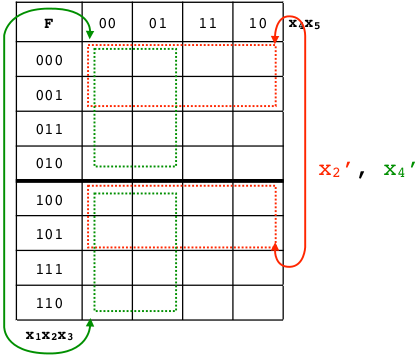
\includegraphics[height=5cm]{ch4/image12}
	\end{figure}


Ainsi, pour une K-Map à $n$ variables:
\begin{enumerate}
	\item $n$-cube de taille 1: $n$ variables (minterme)
	\item $n$-cube de taille 2: $n$-1 variables (on a pu simplifier 1 variable)
	\item $n$-cube de taille 4: $n$-2 variables (on a pu simplifier 2 variables)
	\item $n$-cube de taille 8: $n$-3 variables (on a pu simplifier 3 variables)
	\vdots
	\item $n$-cube de taille $2^n$: constante
\end{enumerate}
\section{Simplification des fonctions logiques avec les K-Maps}
\textit{Consiste à trouver le plus petit nombre des plus grands sous-cubes permettant de couvrir tous les «1» dans une K-Map}\\
On remarque 2 choses importantes:
\begin{itemize}
	\item \textit{[...] le plus petit nombre des sous-cube [...]} : Pour une SdP, influencer la taille de la porte OU et le nombre de portes ET
	\item \textit{[...] les plus grands sous-cubes [...]} : influence la taille de chaque porte ET
\end{itemize}
\paragraph{Implicant premier} est défini comme un sous-cube qui n'est défini au sein d'aucun autre sous-cube
\paragraph{Implicant premier essentiel} est le seul implicant premier à couvrir (au moins) un «1» de la fonction logique $F$

\paragraph{Fonction logique simplifiée} est représentée comme une somme de :
\begin{itemize}
	\item tous les implicants premiers essentiels
	\item certains implicants premiers de façon à couvrir tous les «1» d'une K-Map
\end{itemize}
\subsection{Méthode de simplification (algorithme)}
\begin{enumerate}
	\item Rechercher tous les implicants premiers de la fonction logique écrite sous forme d'une K-Map
	\item Parmi tous les implicants premiers de la fonction, isoler les implicants premiers essentiels 
	\item Couvrir le reste des «1» avec le moins d'implicants premiers possible
\end{enumerate}
\subsection{Remarque}
\subsubsection{Superposition des sous-cubes}
\begin{figure}[H]
	\centering
	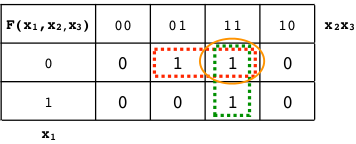
\includegraphics[scale=0.6]{ch4/image13}
\end{figure}
Doit-on superposer le vert et le rouge ou est-il préférable de faire un sous-cube de taille 1?\\
Nous pouvons ($x+x=x$) et nous devons superposer les sous-cubes car :
\begin{equation}
	\begin{array}{cc}
		\text{avec} & \text{sans} \\
		x_1'x_3+x_2x_3 & x_1'x_3+x_1x_2x_3
	\end{array}
\end{equation}
Superposer simplifie donc l'expression
\begin{figure}[H]
	\centering
	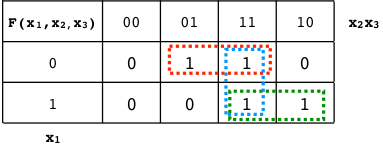
\includegraphics[scale=0.6]{ch4/image14}
\end{figure}
Doit-on inclure le sous-cube bleu?\\
Non car le bleu ne couvre aucun «1» qui ne serait pas encore couvert.
\paragraph{Remarque :} Nous verrons qu'il existe des cas où il faut les inclure.
\subsubsection{Fautes graves}
Entraînera un 0 pour l'exercice :
\begin{itemize}
	\item Ne pas respecter l'adjacence dans la création de la K-Map (lignes et colonnes ne peuvent différer que 1! bit)
	\item Faire des groupements des mintermes adjacents (ex : regrouper les colonnes 1 et 3...)
	\item Faire des groupements de mintermes par 3, 5, 6, 7,... (i.e. construire des sous-cubes qui ne sont pas $2^n$)
\end{itemize}
\section{Fonctions non-complètement spécifiées}
Pour certaines combinaisons de valeur des variables, on ne se préoccupe pas du résultat de la fonction:
\begin{itemize}
	\item Soit parce qu'on se fout de la sortie de ces combinaisons $\rightarrow$ \textbf{don't care}
	\item Soit parce que ces combinaisons n'arriveront jamais $\rightarrow$ \textbf{don't happen}
\end{itemize}
Que ce soit l'un ou l'autre, ils seront marqués par un - . On pourra choisir la valeur (0 ou 1) pour simplifier au mieux l'expression finale.\\

Il faut néanmoins souligner que contrairement au \textit{don't happen} qui ne produira pas de sortie vu que ses combinaisons n'arriveront pas, le \textit{don't care} produira une sortie.

\begin{figure}[H]
	\begin{minipage}{0.5\textwidth}
		\centering
		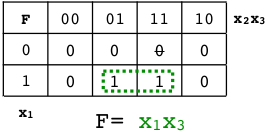
\includegraphics[width=.7\textwidth]{ch4/image15}
	\end{minipage}
	\begin{minipage}{0.5\textwidth}
		\centering
		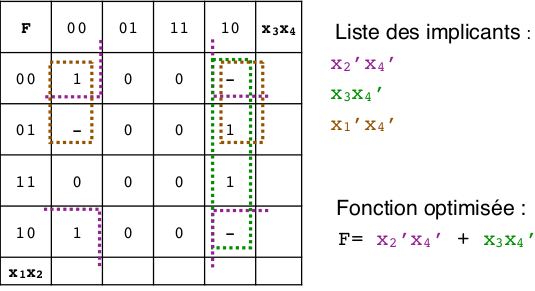
\includegraphics[width=\textwidth]{ch4/image16}
	\end{minipage}
\end{figure}